\documentclass{physlab}

\begin{document}
\begin{titlepage}
\center % Center everything on the page
 
%----------------------------------------------------------------------------------------
%	HEADING SECTIONS
%----------------------------------------------------------------------------------------

\textsc{\LARGE Московский\\[-0.2cm]Физико-Технический Институт\\[0.1cm]\large (государственный университет)}\\[1.5cm] % Name of your university/college
\textsc{\Large Кафедра общей физики}\\[0.1cm] % Major heading such as course name
\textsc{\large Лабораторная работа № 1.2}\\[0.5cm] % Minor heading such as course title

%----------------------------------------------------------------------------------------
%	TITLE SECTION
%----------------------------------------------------------------------------------------

\HRule
\\[0.6cm]
{\huge \bfseries Эффект Комптона}
\\[0.3cm] % Title of your document
\HRule
\\[1.5cm]


 
%----------------------------------------------------------------------------------------
%	AUTHOR SECTION
%----------------------------------------------------------------------------------------

\begin{minipage}[t]{0.48\textwidth}
	\begin{flushleft} \large
		\textsf{Студент}
		
		Ришат \textsc{Исхаков} \\[-0.15cm]
		512 группа

	\end{flushleft}
\end{minipage}
\hfill
\begin{minipage}[t]{0.48\textwidth}
	\begin{flushright} \large
		\textsf{Преподаватель}		
		
		Лев Владиславович \\[-0.15cm]
		\textsc{Инжечик} 

	\end{flushright}
\end{minipage}

\begin{bottompar}
	\begin{center}
		
\includegraphics[width = 80 mm]{logo.jpg}
	\end{center}
	\today

\end{bottompar}
\vfill % Fill the rest of the page with whitespace

\end{titlepage}

\paragraph{Цель работы:} С помощью сцинтилляционного спектрометра исследуется энергетический спектр $\gamma$-квантов, рассеянных на графите. Определяется энергия рассеянных $\gamma$-квантов в зависимости от угла рассеяния, а также энергия покоя частиц, на которых происходит комптоновское рассеяние.

\section{Теория}
Будем считать, что $\gamma$-излучение~---~поток квантов с энергией $\hbar\omega$ и импульсом $p=\frac{\hbar\omega}{c}$. Эффект Комптона~---~увеличение длины волны рассеянного излучения по сравнению с падающим~---~как результат упругого соударения  $\gamma$-кванта и свободного электрона.
	
Пусть до соударения электрон покоился ($mc^2$), а  $\gamma$-квант имел энергию~$\hbar\omega$ и импульс~$p=~\frac{\hbar\omega}{c}$.

Тогда после соударения:
\[ E_\text{электрона}=\gamma mc^2 \]
\[ p_\text{электрона}=\gamma mv \]
\[ \gamma=\sqrt{\dfrac{1}{1-\frac{v^2}{c^2}}}, \]
а  $\gamma$-квант рассеивается на угол~$\theta$ по отношению к начальному движению:

\begin{figure}[H] 
\begin{minipage}[H]{0.48 \lw}
    \centering
    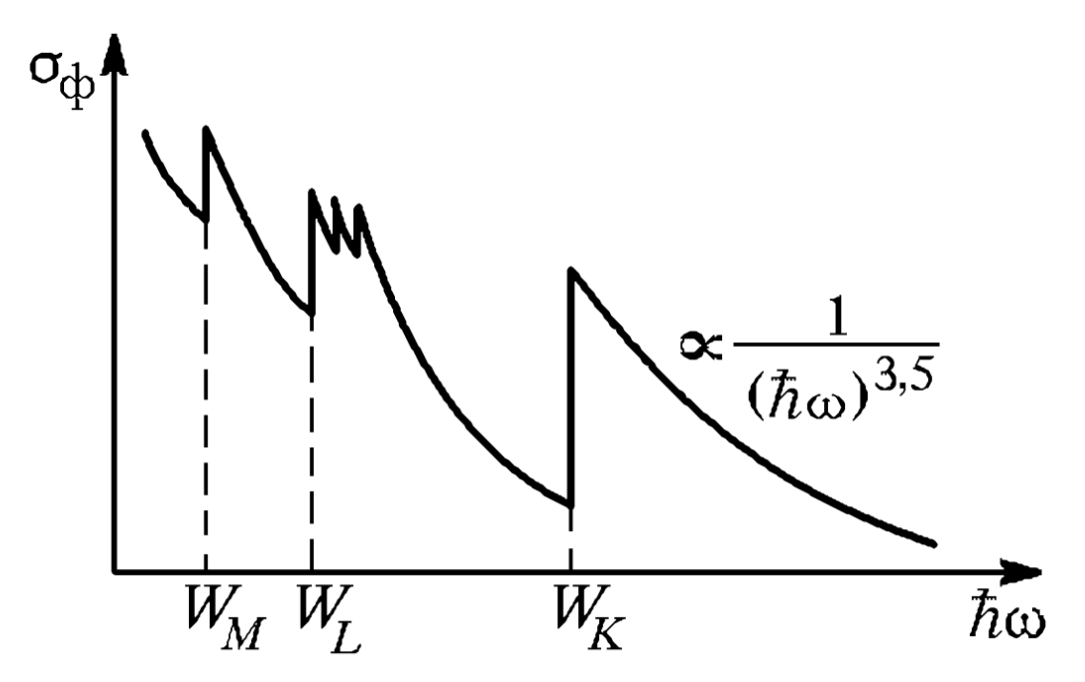
\includegraphics[width=0.8\linewidth]{01}
    \caption{Векторная диаграмма рассеяния}
\end{minipage}
\hfill
\begin{minipage}[H]{0.48 \lw}
\begin{align}
    &E_\gamma = \hbar\omega_1 \\
    &p_\gamma = \frac{\hbar\omega_1}{c} \\
    \text{ЗСЭ: }& mc^2+\hbar \omega_0 = \gamma mc^2+\hbar \omega_1 \\
    \text{ЗСИ: }& \frac{\hbar\omega_0}{c} = \frac{\hbar\omega_1\cos\theta}{c}+\gamma mvcos\varphi \\
    &\gamma mvsin\varphi = \frac{\hbar\omega_1}{c}sin\theta
\end{align}     
\end{minipage}
\end{figure}

Переходя от $\omega_0$, $\omega_1$ к $\lambda_0$, $\lambda_1$:

\begin{equation}
\Delta\lambda=\lambda_1-\lambda_0=\dfrac{h}{mc}(1-\cos\theta)=\Lambda_k(1-\cos\theta)
\label{eq:goal}
\end{equation}
	
$\Lambda_k = \dfrac{h}{mc} = 2.42\cdot 10^{-10}$ \cm~---~комптоновская $\lambda$ электрона.

При рассеянии квантов невысокой ($ 1 \div 10 \K \eV$) энергии часть электронов ведёт себя как связанные, а часть~---~как свободные, т.е. одновременно наблюдаются релеевское и комптоновское рассеяния.
		
Цель работы~---~проверка соотношения \eqref{eq:goal}. Его можно преобразовать от длин волн к энергии квантов:
\[\frac{1}{\varepsilon(\theta)}-\frac{1}{\varepsilon_0}=1-\cos\theta, \quad \varepsilon_0=\frac{E_0}{mc^2} \]

\section{Экспериментальная установка}

\begin{figure}[H]
\centering
    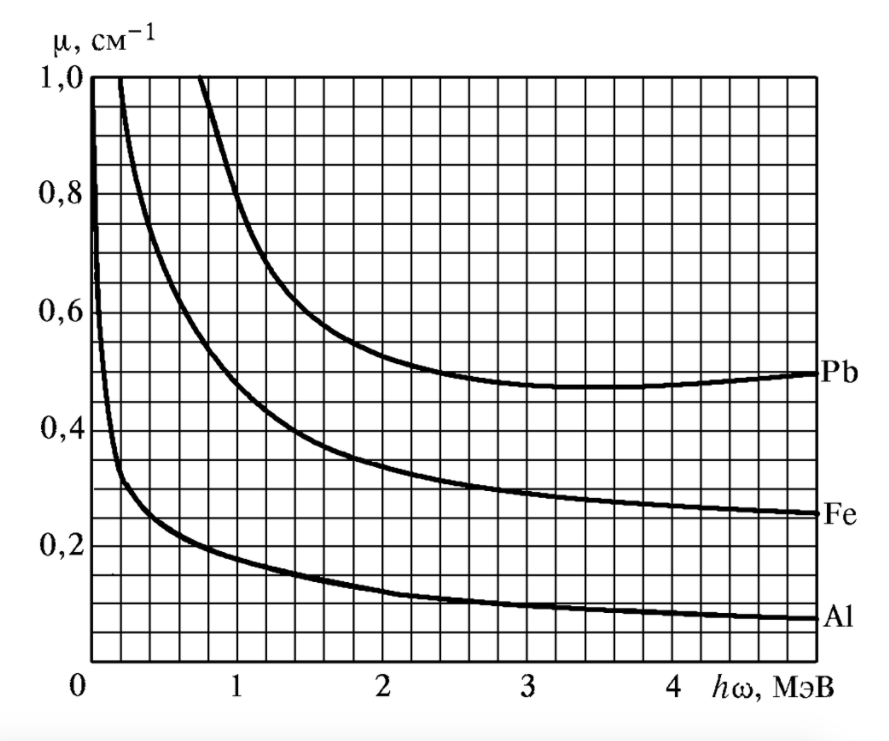
\includegraphics[width=0.6\linewidth]{02}
\caption{Блок~-~схема установки по изучению рассеяния $\gamma$-квантов: 1~-~источник излучения ($^{137}Cs$), 2~-~графитовая мишень, 3~-~фотоэлектронный умножитель (ФЭУ), 4~-~сцинтиллятор, 5~-~свинцовый коллиматор, 6~-~лимб}
\end{figure}

\begin{figure}[H]
\centering
    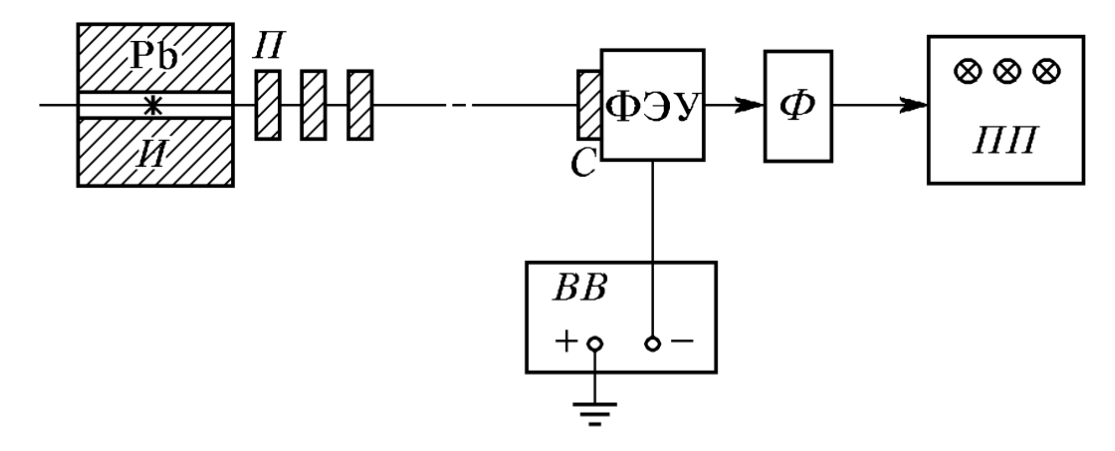
\includegraphics[width=0.4\linewidth]{03}
\caption{Блок~-~схема измерительного комплекса: Д~-~дисплей, ПР~-~принтер, ВСВ~-~высоковольтный выпрямитель, УА~-~усилитель~-~анализатор, КЛ~-~клавиатура}
\end{figure}

%Источник излучения испускает $\gamma$-лучи с энергией 662 кэВ. Кванты, испытавшие комптоновское рассеяние в мишени, регистрируются сцентилляционным счётчиком.

\section{Ход работы}
	Устанавливая сцинтилляционный счётчик под разными углами $\theta$ к первоначальному направлению полёта $\gamma$-квантов, сняли амплитудные спектры и определили положение фотопиков для каждого угла.
	
\begin{table}[H]
\centering
\caption{Результаты измерений:}
\begin{tabular}{|l|c|c|c|c|c|c|c|c|c|c|c|c|c|}
\hline
Угол,$^\circ$ & 0 & 11 & 20 & 30 & 40 & 50 & 60 & 70 & 80 & 90 & 100 & 110 & 120 \\ \hline
Канал & 986 & 891 & 803 & 734 & 691 & 603 & 526 & 502 & 440 & 414 & 370 & 349 & 316 \\ \hline
\end{tabular}
\end{table}
			
\section{Обработка данных}

\begin{enumerate}
	\item Построили график зависимости $\dfrac{1}{N(\theta)}$ от $(1-\cos\theta)$ и провели через точки наилучшую прямую:			
    \begin{figure} [H]
    	\centering
        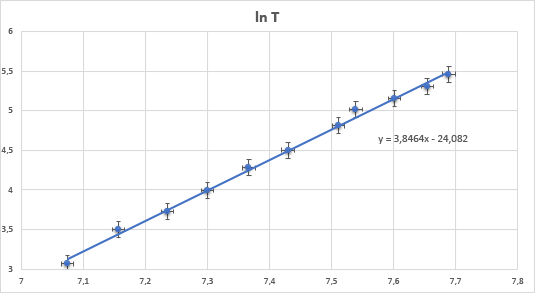
\includegraphics[width=0.7\linewidth]{graph}
        \caption{График зависимости $\dfrac{1}{N(\theta)}-\dfrac{1}{N(0)}= A(1-\cos\theta)$}
    \end{figure}
		Погрешности аппроксимации, рассчитанные методом наименьших квадратов: ($y=Ax+b$): $\frac{\sigma A}{A} \approx 0.023$; $\frac{\sigma b}{b} \approx 0.014$.
		
	\item С помощью графика определили коэффициент пропорциональности между N($\theta$) и $\varepsilon(\theta)$: A = $\frac{\varepsilon}{N}\approx 0.0013$.
				
	\item Перейдя от переменной $\varepsilon=\frac{E}{mc^2}$ к энергии E, получаем, что энергия частицы, на которой происходит рассеяние, находится по формуле:
\[ mc^2=E_\gamma\cdot\dfrac{N(90)}{N(0)-N(90)}, \]
	   где $E_\gamma$~---~энергия $\gamma$-лучей, рассеянных источником.
		
		При этом значения  $N(0)$ и $N(90)$ используем полученные из графика (а не полученные непосредственно при измерениях), так как эти значения учитывают измерения, сделанные под другими углами.
\[N_\text{наил.}(0)\approx909.09, \quad N_\text{наил.}(90)\approx416.67 \]
	Полученная энергия:
\[ E_{\text{эксп.}} = mc^2 = 662 \; \K \eV \cdot \frac{416.67}{909.09-416.67} \approx 560 \; \K \eV \]	
	\item Рассчитаем погрешности измерений:
        \[\dfrac{\sigma N(0)}{N(0)}=\dfrac{\sigma b}{b}\approx0.014 \]
        \[\dfrac{\sigma N(90)}{N(90)}=\sqrt{\left(\frac{\sigma b}{b}\right)^2 + \left(\frac{\sigma A}{A}\right)^2}=\sqrt{(0.014)^2 + (0.023)^2} \approx 0.027 \]
        \[\dfrac{\sigma E}{E}=\sqrt{\left(\frac{\sigma N(90)}{N(90)}\right)^2+\left(\frac{\sigma N(0)+\sigma N(90)}{N(0)-N(90)}\right)^2} = \sqrt{(0.027)^2+\left(\frac{11.25+12.73}{909.09-416.67}\right)^2} \approx 0.056=5.6 \% \]
        
	
	С учётом погрешностей:
	\[ E_{\text{эксп.}} = 560 \pm 32 \; \K \eV \]
	Энергия покоя электрона:
	\[ E_{\text{электр.}}=mc^2=9.1\cdot 10^{-31}\cdot (3\cdot 10^8)^2 \approx 511 \; \K \eV\]
	\end{enumerate}

\section{Вывод}

Исследовали энергетический спектр $\gamma$-квантов, рассеянных на графите.  Используя полученные данные, построили график зависимости $\frac{1}{N(\theta)}$ от $(1-\cos\theta)$, где N - номер канала в анализаторе, $\theta$ - угол рассеяния. Полученная зависимость оказалась линейная. С её помощью определили энергию покоя частицы, на которой происходит рассеяние: $E_{\text{эксп.}}=560\pm32 \; \K \eV$. В пределах погрешностей полученная величина оказалась близкой к энергии покоя электрона: $E_{\text{электр.}}\approx511 \; \K \eV$, то есть, как и предполагалось, рассеяние происходит на электронах. Погрешность вычисления энергии составила $5.6\%$.
	

\end{document}